\chapter{METODE DAN RANCANGAN PENELITIAN}

\section{Deskripsi Umum Penelitian}
Penelitian dilakukan melalui pengembangan prototipe dan evaluasi eksperimental terkontrol. Prototipe menerima aturan interaksi serta ekspor observasi, membentuk graf kausal per alur kerja, memeriksa aturan, dan menghasilkan keputusan beserta penjelasan. Alur pemesanan digunakan sebagai objek uji yang menyediakan pembayaran dan reservasi persediaan konkuren sebelum pengiriman.

Pemeriksaan utama menggunakan semantik eksistensial pada Persamaan~\ref{eq:existential}. Pencarian dilakukan pada kombinasi himpunan peristiwa yang sudah diproses dan state model workflow. Prototipe pendahuluan yang memeriksa keterjangkauan kausal merupakan bahan awal, bukan implementasi selesai untuk semantik ini.

\begin{figure}[H]
  \centering
  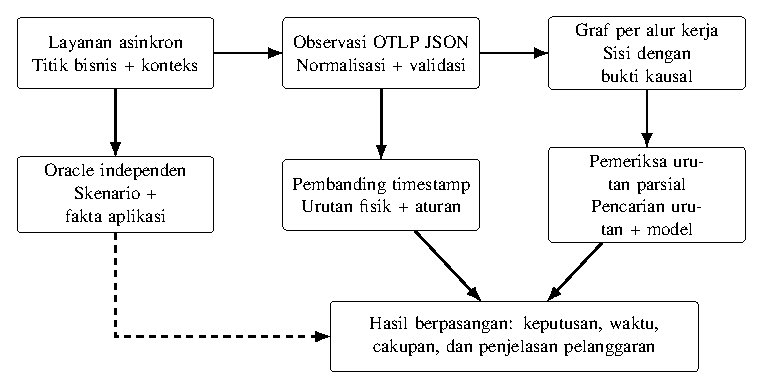
\includegraphics[width=\textwidth]{architecture-overview}
  \caption{Rancangan alur observasi dan dua pendekatan pemeriksaan pada masukan yang sama. Oracle menentukan label dari skenario dan fakta aplikasi, bukan dari keluaran verifier.}
  \label{fig:architecture}
\end{figure}

\section{Tahapan Penelitian}
Tahapan penelitian ditunjukkan pada Gambar~\ref{fig:methodology} dan dijelaskan sebagai berikut.
\begin{enumerate}
  \item Penelaahan literatur dan penetapan semantik. Kegiatan mencakup penelaahan sumber terkait, pemilihan aturan, serta pemisahan dependensi kausal dari penerimaan suatu urutan sekuensial.
  \item Penyusunan kontrak observasi. Titik bisnis, identitas alur kerja, arah sisi, serta jaminan kelengkapan ditetapkan sebelum penyusunan dataset.
  \item Pengembangan prototipe. Adapter OTLP JSON, normalisasi peristiwa, pembentukan graf, pemeriksaan aturan, dan penjelasan deterministik disusun sebagai komponen terpisah.
  \item Penyiapan objek uji dan baseline. Layanan terkontrol menghasilkan variasi eksekusi, sedangkan baseline menerapkan pemeriksaan urutan timestamp terhadap aturan yang sama.
  \item Kalibrasi dan penyusunan korpus. Label diperiksa melalui skenario dan fakta aplikasi. Uji awal memastikan perubahan jam tidak mengubah graf, serta kehilangan observasi tidak disamakan dengan event bisnis hilang.
  \item Pelaksanaan eksperimen. Kedua pendekatan dijalankan pada masukan berpasangan. Data keputusan, waktu, ukuran graf, dan penjelasan dicatat.
  \item Analisis dan pelaporan. Hasil ditafsirkan per skenario, keterbatasan dicatat, dan artefak disiapkan agar eksperimen dapat diulang.
\end{enumerate}

\begin{figure}[H]
  \centering
  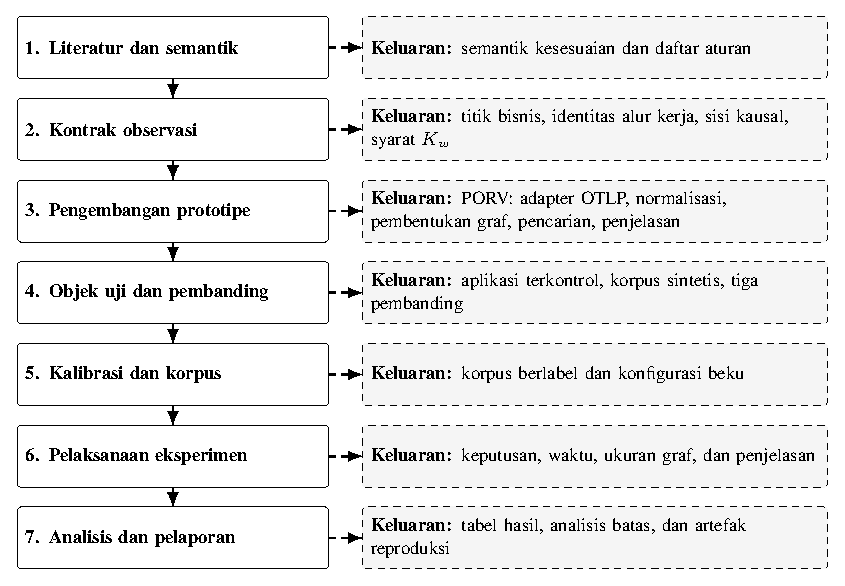
\includegraphics[width=0.8\textwidth]{experiment-flow}
  \caption{Tahapan penelitian, dengan kalibrasi sebelum pengukuran resmi.}
  \label{fig:methodology}
\end{figure}

\section{Kontrak Observasi dan Pembentukan Graf}
\subsection{Unit Peristiwa dan Identitas Alur Kerja}
Setiap peristiwa dinormalisasi menjadi record yang memuat identitas unik, jenis peristiwa, layanan, identitas trace/span, identitas alur kerja, dan referensi pendahulu. Timestamp dipertahankan untuk baseline dan penjelasan, tetapi tidak digunakan untuk menyimpulkan sisi lintas layanan. Satu peristiwa bisnis tidak boleh diam-diam dipetakan menjadi beberapa peristiwa yang dihitung sebagai aksi berbeda.

Peristiwa bisnis direkam pada titik yang ditetapkan kontrak. Keberhasilan pembayaran dan reservasi persediaan, misalnya, dicatat setelah perubahan aplikasi berhasil disimpan. Span durasional yang sudah ada tetap dapat menjadi konteks, tetapi awal permintaan tidak menggantikan titik keberhasilan. Pemilihan titik ini diuji melalui fakta aplikasi, bukan hanya nama span.

Pengelompokan dilakukan menurut atribut bisnis, misalnya \kode{order.id}. Peristiwa antara, yang tidak cocok dengan alias aturan, tetap disimpan karena dapat menjadi bagian lintasan kausal. Referensi lintas pesanan tidak ditelusuri sebagai dependensi yang sah. Referensi tersebut ditandai sebagai cacat bukti, sehingga tidak terjadi pemenuhan prasyarat dari pesanan lain.

\subsection{Sumber Sisi yang Diterima}
Graf $G_w=(V_w,D_w)$ dibentuk per alur kerja. Sisi $D_w$ diterima dari sumber berikut.
\begin{enumerate}
  \item Urutan eksekusi lokal yang dijamin instrumentasi. Peristiwa pada satu urutan eksekusi diberi nomor urut atau referensi pendahulu. Kesamaan layanan tanpa jaminan satu urutan eksekusi tidak cukup, karena satu proses dapat menangani pekerjaan konkuren.
  \item Hubungan awal span induk menuju awal span anak sesuai konteks yang diketahui. Hubungan tersebut tidak diperluas menjadi urutan akhir induk terhadap seluruh peristiwa anak.
  \item Hubungan pengiriman menuju pemrosesan pesan dengan identitas pesan dan konteks yang cocok, sesuai kontrak propagasi \citep{otelmessaging}.
  \item Link atau referensi pendahulu yang secara eksplisit diberi makna kausal dalam instrumentasi aplikasi. Link umum yang semantiknya tidak ditetapkan tidak digunakan sebagai sisi berarah \citep{otelapi}.
\end{enumerate}

Dalam prototipe, atribut seperti \kode{porv.predecessors} dan penanda \kode{porv.causal} dapat digunakan sebagai kontrak aplikasi. Keduanya bukan field semantik standar OpenTelemetry. Penggunaan struktur OTLP standar dengan atribut tambahan harus dilaporkan secara jujur sebagai instrumentasi eksplisit, bukan klaim bahwa tracing otomatis sudah merekam seluruh kausalitas.

\subsection{Validasi Masukan dan Kelengkapan}
Normalisasi memeriksa identitas duplikat, nilai korelasi, referensi yang tidak terselesaikan, dan siklus. Ekspor tidak sesuai skema dipisahkan sebagai kesalahan masukan. Graf yang mengandung siklus tidak dipaksa menjadi \ist{partial order}; keputusan urutan dinyatakan tidak dapat disimpulkan hingga masalah observasi dijelaskan.

Penanda kelengkapan $K_w$ hanya diberikan pada pengumpulan alur kerja secara terkontrol apabila semua titik bisnis dan referensi kausal yang diperlukan telah terkumpul serta tidak ada kehilangan yang diketahui. Penutupan permintaan atau waktu akhir span tidak membuktikan $K_w$. Pada uji kehilangan telemetri, penanda kelengkapan dicabut dan jumlah atau referensi kehilangan disimpan.

Pembentukan graf dan pemeriksaan siklus memerlukan waktu $O(|V_w|+|D_w|)$. Biaya pencarian kesesuaian berbeda: banyaknya kombinasi peristiwa dan state dapat tumbuh eksponensial. Penelitian tidak menyamakan replikasi banyak graf kecil dengan satu workflow besar yang memiliki banyak pilihan urutan.

\section{Representasi Workflow dan Algoritma Pemeriksaan}
\subsection{State Machine yang Didukung}
Spesifikasi awal berupa deterministic finite automaton $P=(Q,\Sigma,\delta,q_0,F)$: himpunan state, alfabet peristiwa bisnis, fungsi transisi parsial, state awal, dan state penerima. Transisi yang tidak didefinisikan menolak langkah tersebut. Setiap observasi yang dinyatakan lengkap mewakili satu workflow tertutup; state akhir harus termasuk $F$. Kebijakan untuk workflow yang berhenti secara sah, pembatalan, atau percobaan ulang ditulis sebagai transisi dan state penerima tersendiri bila dibutuhkan aplikasi.

Listing~\ref{lst:rules} menunjukkan contoh konseptual yang format finalnya ditetapkan saat implementasi. Model menerima pembayaran dan reservasi dalam dua urutan, kemudian satu pengiriman. Transisi pengiriman kedua tidak tersedia. Nama simbol dipetakan secara eksplisit ke titik bisnis dan identitas pesanan.
\begin{lstlisting}[language=yaml,caption={Contoh state machine workflow pemesanan},label={lst:rules}]
name: checkout
correlation: order.id
initial: new
accepting: [completed]
events:
  created: order.created
  paid: payment.succeeded
  reserved: stock.reserved
  shipped: shipping.started
transitions:
  - [new, created, opened]
  - [opened, paid, paid_only]
  - [opened, reserved, reserved_only]
  - [paid_only, reserved, ready]
  - [reserved_only, paid, ready]
  - [ready, shipped, completed]
\end{lstlisting}

Model contoh tidak diasumsikan berlaku langsung pada aplikasi eksternal. Model mengikuti perilaku aplikasi yang dipilih; percobaan pesan yang berulang tidak otomatis sama dengan pengiriman bisnis yang berulang. Peristiwa konteks diberi label $\epsilon$ dan tidak mengubah state, tetapi tetap dijadwalkan sesuai graf. Semua peristiwa bisnis relevan harus tercakup dalam pemetaan yang dibekukan sebelum eksperimen.

\subsection{Keputusan Berdasarkan Bukti}
\begin{table}[H]
  \centering\small
  \caption{Dasar keputusan kesesuaian workflow}
  \label{tab:verdict}
  \begin{tabularx}{\textwidth}{@{}p{2.6cm}XX@{}}
    \toprule
    Status & Kondisi & Batas interpretasi \\
    \midrule
    Konsisten & Bukti lengkap dan ada urutan topologis yang diterima model & Ada penjelasan yang diizinkan; tidak menjamin semua urutan benar \\
    Tidak konsisten & Bukti lengkap dan pencarian tuntas membuktikan tidak ada urutan yang diterima & Ketidaksesuaian observasi terhadap model, bukan semua properti aplikasi \\
    Tidak dapat disimpulkan & Bukti tidak lengkap/ambigu, graf bermasalah, atau pencarian mencapai batas sumber daya & Tidak dihitung sebagai penerimaan ataupun penolakan \\
    \bottomrule
  \end{tabularx}
\end{table}

Pembayaran dan pengiriman yang tidak terurut dapat dinyatakan konsisten jika model menerima pembayaran lebih dahulu. Ketiadaan lintasan pembayaran menuju pengiriman tidak lagi dijadikan pelanggaran tersendiri. Sebaliknya, sisi pengiriman menuju pembayaran memaksa urutan yang ditolak model contoh. Bukti tidak lengkap tidak diperlakukan sebagai workflow lengkap yang tinggal diurutkan ulang. Kesalahan format dilaporkan terpisah; tidak ada klaim umum bahwa subsekuens yang ditolak tetap ditolak setelah peristiwa yang hilang ditambahkan.

\subsection{Pencarian Urutan yang Diterima}
Konfigurasi pencarian adalah $(S,q)$, dengan $S\subseteq V_w$ himpunan peristiwa yang sudah diproses dan $q\in Q$ state model. Pencarian dimulai dari $(\varnothing,q_0)$. Peristiwa $v\notin S$ dapat dipilih hanya jika semua pendahulu langsungnya termasuk $S$. Jika $\lambda(v)=\epsilon$, state tidak berubah; jika simbol bisnis, transisi $\delta(q,\lambda(v))$ harus tersedia. Langkah menghasilkan $(S\cup\{v\},q')$.

Jika $S=V_w$ dan $q\in F$, pencarian berhenti dengan satu urutan saksi yang diterima. Jika seluruh konfigurasi yang dapat dicapai sudah dieksplorasi tanpa saksi, observasi tidak konsisten. Memoisasi berdasarkan pasangan $(S,q)$ mencegah eksplorasi ulang konfigurasi yang sama; urutan kandidat menurut identitas menghasilkan saksi deterministik. Batas waktu dan konfigurasi dicatat sebelum eksperimen. Pencarian yang terhenti karena batas tersebut menghasilkan tidak dapat disimpulkan, bukan tidak konsisten.

Batas atas kasar jumlah konfigurasi adalah $2^{|V_w|}|Q|$, dengan sampai $|V_w|$ kandidat pada setiap konfigurasi. Batasan kausal mengurangi himpunan yang dapat dicapai, tetapi lebar konkurensi dapat memperbesar pencarian. Optimasi tambahan hanya diterapkan setelah kesetaraan keputusan diperiksa terhadap pencarian acuan pada graf kecil; klaim waktu polinomial atau pengurangan urutan tanpa bukti tidak dibuat.

\section{Baseline Urutan Timestamp}
Baseline memakai peristiwa, pemetaan simbol, model state machine, dan gerbang kualitas bukti yang sama. Peristiwa diurutkan menaik menurut timestamp fisik, dengan identitas sebagai pemutus seri tetap. Model menjalankan satu kata hasil proyeksi urutan tersebut: diterima jika semua transisi tersedia dan state akhir menerima. Baseline tidak mencari alternatif jika kata itu ditolak.

Timestamp hilang atau tidak dapat dibaca menghasilkan tidak dapat disimpulkan untuk baseline. Urutan timestamp yang bertentangan dengan sisi kausal ditandai dalam laporan, tetapi tidak diperbaiki menggunakan graf; perlakuan ini merepresentasikan baseline pengurutan waktu fisik secara langsung. Pengurutan waktu yang diperbaiki agar mengikuti graf merupakan baseline lain dan tidak dicampur dengan baseline utama.

Pada graf lengkap yang sama, jika urutan timestamp adalah urutan topologis dan diterima model, verifier eksistensial juga harus menerima. Karena itu, perbedaan berupa baseline menerima tetapi verifier menolak memerlukan urutan timestamp yang bertentangan dengan kausalitas atau kesalahan implementasi. Konkurensi dapat memberi penolakan baseline jika urutan timestamp bukan urutan yang diizinkan padahal alternatif kompatibel diterima. Namun, bila model menerima semua pertukaran peristiwa independen, konkurensi saja tidak memberi keuntungan. Dampak ini diuji, bukan diasumsikan berlaku pada setiap workflow.

\section{Rancangan Penjelasan Ketidaksesuaian}
Penerimaan menyertakan satu urutan saksi. Penolakan menyertakan model, identitas workflow, peristiwa relevan, batasan urutan, serta ringkasan pencarian tuntas. Satu urutan yang gagal bukan counterexample yang cukup untuk semantik eksistensial karena urutan lain mungkin diterima. Ringkasan eksplorasi pada graf penuh menjadi dasar kesimpulan, sementara irisan peristiwa hanya membantu penjelasan.

Kasus sederhana seperti pengiriman yang diketahui mendahului pembayaran dapat ditampilkan bersama lintasan dan transisi yang bertentangan. Jika alasan ringkas belum dapat diperoleh dengan benar, seluruh graf workflow dilaporkan. Tidak diklaim adanya counterexample minimal atau bahwa subgraf penjelasan selalu membuktikan ketidaksesuaian secara mandiri. Ukuran penjelasan tetap diukur sebagai keluaran pendukung, dengan kebenaran dan batas maknanya diperiksa lebih dahulu.

\section{Lingkungan dan Bahan Penelitian}
Implementasi awal direncanakan memakai TypeScript/Bun dengan pemisahan adapter, graf, aturan, dan pemformat keluaran. Objek uji terdiri atas empat proses layanan dengan penyimpanan lokal terpisah. Aksi pembayaran merupakan simulasi dan tidak memakai penyedia pembayaran atau transaksi keuangan nyata.

Prototipe pendahuluan pada workspace peneliti menyediakan dasar pemeriksaan \ist{offline} dan demo alur pemesanan dengan proses terpisah. Demo tersebut menghasilkan struktur OTLP JSON melalui eksportir eksplisit; hal itu belum sama dengan pembuktian interoperabilitas terhadap keluaran SDK. Sebagai bagian penelitian, setidaknya satu jalur ekspor dari SDK OpenTelemetry yang dipilih akan diuji terhadap adapter. Versi SDK, Bun, dependensi, dan profil konvensi dikunci sebelum pengumpulan data resmi.

Spesifikasi perangkat, sistem operasi, versi runtime, konfigurasi instrumentasi, dan konfigurasi eksportir akan dicatat pada manifest eksperimen. Nilai perangkat keras tidak ditetapkan sebelum mesin eksperimen dipilih. Demo HTTP konkuren digunakan untuk kasus dasar. Evaluasi penerapan menggunakan setidaknya satu aplikasi microservices sumber terbuka pihak lain yang memiliki workflow berbasis pesan dan dapat diinstrumentasi. Target awal kedua aplikasi eksternal bergantung pada studi kelayakan; pengurangan cakupan dilaporkan. Pemilihan mencatat revisi, lisensi, kebutuhan sumber daya, model yang sesuai perilaku asli, serta patch instrumentasi dan fault. Hasil aplikasi eksternal dianalisis terpisah dari demo dan graf sintetis.

\section{Skenario dan Label Acuan}
\label{sec:scenarios}
Dua label acuan disimpan terpisah. Label kesesuaian observasi menyatakan ada atau tidaknya urutan yang diterima model. Untuk graf kecil, label ini ditentukan oleh enumerasi independen seluruh urutan topologis dan pemeriksaan model, bukan pencarian termemoisasi yang dievaluasi. Kasus lebih besar menggunakan konstruksi dengan saksi yang diketahui atau kontradiksi yang dapat dibuktikan independen; label yang belum terverifikasi tidak dimasukkan ke akurasi utama.

Label perilaku aplikasi berasal dari skenario, catatan aksi, dan fakta penyimpanan. Pelanggaran aplikasi dapat tetap konsisten dengan observasi bila observasi mengizinkan penjelasan lain; kasus tersebut dilaporkan sebagai keterbatasan kemampuan deteksi terhadap perilaku nyata, bukan diberi label tidak konsisten secara paksa. Oracle tidak memakai hasil verifier sebagai label.

\begin{longtable}{@{}p{0.7cm}p{3.0cm}p{6.1cm}p{2.8cm}@{}}
  \caption{Skenario uji dan label kesesuaian observasi}\label{tab:scenarios}\\
  \toprule ID & Skenario & Perlakuan & Acuan \\
  \midrule\endfirsthead
  \toprule ID & Skenario & Perlakuan & Acuan \\
  \midrule\endhead
  S1 & Sekuensial sesuai & Graf mengikuti kata yang diterima model & Konsisten \\
  S2 & Konkuren sesuai & Pembayaran dan reservasi dapat bertukar urutan; model menerima keduanya & Konsisten \\
  S3 & Pergeseran jam & Timestamp diubah; peristiwa dan sisi dari S2 tetap & Konsisten \\
  S4 & Transisi dini terbukti & Graf memaksa pengiriman sebelum pembayaran & Tidak konsisten \\
  S5 & Aksi wajib hilang & Pembayaran/reservasi tidak dilakukan; observasi workflow tertutup lengkap & Tidak konsisten \\
  S6 & Aksi duplikat & Dua pengiriman bisnis nyata; model hanya menerima satu & Tidak konsisten \\
  S7 & Urutan terbuka & Pembayaran dan pengiriman tidak terurut; ada urutan pembayaran lebih dahulu & Konsisten, bukan bukti kausal \\
  S8 & Kehilangan telemetri & Aksi aplikasi tetap; peristiwa/sisi ekspor dihapus dan kelengkapan dicabut & Tidak cukup bukti \\
  S9 & Bukti bermasalah & Referensi rusak, korelasi hilang, atau graf bersiklus & Tidak cukup bukti / kesalahan masukan \\
  S10 & Alternatif workflow & Model mengizinkan dua cabang/transisi; label diuji pada graf kecil dengan beberapa urutan & Sesuai oracle independen \\
  \bottomrule
\end{longtable}

S7 sengaja menguji keputusan eksistensial yang berbeda dari pemeriksa prasyarat kausal. Kasus tambahan mencakup workflow dengan satu urutan diterima dan urutan lain ditolak, serta kegagalan pencarian karena batas sumber daya. S8 membedakan kehilangan observasi dari penghilangan aksi bisnis pada S5. Fault pada aplikasi eksternal dibuat melalui patch atau switch terkontrol, dengan perubahan instrumentasi dan perubahan logika bisnis dicatat terpisah. Replay pesan hanya dilabeli pelanggaran bisnis jika benar-benar menghasilkan efek yang dilarang model aplikasi.

\section{Desain Eksperimen dan Protokol Pengukuran}
\subsection{Variabel dan Korpus}
Variabel utama adalah pendekatan pemeriksaan: pencarian urutan kompatibel atau urutan timestamp tunggal. Faktor yang divariasikan meliputi jenis skenario, jumlah peristiwa, lebar cabang konkuren, ukuran state machine, panjang lintasan, kepadatan sisi, pergeseran jam, dan kualitas bukti. Aturan, input normalisasi, mesin, serta kondisi proses dijaga sama pada pasangan pengukuran.

Rencana awal menggunakan 30 run atau seed berbeda per keluarga skenario. Angka tersebut merupakan rencana operasional untuk memperoleh variasi yang dapat diperiksa, bukan klaim kecukupan statistik untuk semua efek. Run yang memakai trace sama hanya menambah sampel waktu, bukan menambah jumlah eksekusi independen untuk ketepatan deteksi. Sampel dikelompokkan menurut keluarga dan sumbernya agar hasil tidak didominasi replikasi identik.

Kalibrasi pencarian dimulai pada workflow sekitar 4, 8, 12, 16, dan 20 peristiwa bisnis, dengan lebar cabang 1, 2, 4, dan 8 jika memungkinkan. Beban 100, 500, 1.000, dan 5.000 peristiwa digunakan untuk banyak workflow kecil atau stress test graf yang struktur kausalnya membatasi pilihan; penyelesaian satu workflow besar tidak dijanjikan. Ukuran state machine dan jumlah konfigurasi yang dieksplorasi dicatat. Dua bentuk beban dibedakan: banyak alur kerja independen dan satu alur kerja yang membesar. Kombinasi yang tidak memenuhi jumlah peristiwa atau bentuk graf diberi alasan dan tidak diganti diam-diam.

Pergeseran jam diatur pada 0, $\pm100$ ms, $\pm1$ s, dan $\pm5$ menit. Nilai tersebut merupakan stress test yang dapat direproduksi, bukan perkiraan distribusi jam pada sistem produksi. Kehilangan observasi diuji melalui penghilangan peristiwa relevan dan variasi kehilangan terkontrol dengan seed tetap. Label aplikasi dan label kecukupan bukti disimpan terpisah.

\subsection{Pengumpulan Data}
Untuk setiap run, skenario dijalankan dengan keadaan aplikasi baru. Catatan fakta bisnis dan konfigurasi perlakuan disimpan, telemetri dikumpulkan, lalu kualitas bukti divalidasi. Hasil normalisasi yang sama diberikan kepada kedua pendekatan. Urutan eksekusi pemeriksa diacak atau diseimbangkan untuk mengurangi pengaruh beban dan cache.

Waktu verifikasi inti diukur setelah parsing dan normalisasi selesai. Secara terpisah, waktu menyeluruh dari pembacaan input hingga serialisasi laporan dicatat agar biaya adapter tidak tersembunyi. Setiap konfigurasi waktu menjalani lima pemanasan dan sekurang-kurangnya 30 pengulangan ukur pada proses eksperimen yang dijelaskan. Jika dipilih proses baru per sampel, biaya startup dicatat dan dipisahkan dari durasi inti.

Run yang gagal dijalankan diberi status kegagalan eksperimen dan tidak dihitung sebagai keputusan pemeriksa. Batas waktu ditetapkan sebelum pengukuran; timeout tetap dilaporkan sebagai ketidakberhasilan menyelesaikan pemeriksaan. Pengaturan yang berubah setelah kalibrasi menghasilkan versi korpus atau manifest baru, sehingga sampel dari konfigurasi berbeda tidak tercampur tanpa penjelasan.

\subsection{Metrik Ketepatan dan Cakupan}
Metrik utama mengikuti draft penelitian: ketepatan keputusan, waktu verifikasi, dan ukuran penjelasan. Cakupan serta jumlah konfigurasi pencarian menjadi ukuran pendukung agar abstain dan biaya eksplorasi tidak tersembunyi. Jumlah layanan dan titik bisnis yang membutuhkan tambahan instrumentasi dilaporkan sebagai deskripsi penerapan, bukan klaim overhead aplikasi tanpa eksperimen tersendiri.

Pada korpus lengkap, ketidaksesuaian observasi merupakan kelas positif. True positive ($TP$) menyatakan observasi tidak konsisten yang ditolak benar; false positive ($FP$) menyatakan observasi konsisten yang ditolak; false negative ($FN$) menyatakan observasi tidak konsisten yang diterima; true negative ($TN$) menyatakan observasi konsisten yang diterima. Label menggunakan semantik eksistensial untuk kedua pendekatan. Ketepatan deteksi fault aplikasi dilaporkan terpisah menurut fakta bisnis, termasuk fault yang observasinya masih kompatibel dengan model; dua jenis ketepatan tersebut tidak digabungkan.
\begin{align}
  \operatorname{FPR} &= \frac{FP}{FP+TN}, &
  \operatorname{FNR} &= \frac{FN}{FN+TP}, \\
  \operatorname{Precision} &= \frac{TP}{TP+FP}, &
  \operatorname{Recall} &= \frac{TP}{TP+FN}.
\end{align}
Penyebut nol dilaporkan sebagai tidak terdefinisi, bukan diberi nilai nol. Keputusan tidak dapat disimpulkan dilaporkan di luar matriks biner. Agar pemeriksa tidak tampak akurat hanya karena banyak menahan keputusan, cakupan dinyatakan sebagai:
\begin{equation}
  C=\frac{N_{\mathrm{konsisten}}+N_{\mathrm{tidak\ konsisten}}}{N_{\mathrm{seluruh\ input\ evaluasi}}}.
\end{equation}
Jumlah keputusan benar terhadap seluruh input berlabel juga dilaporkan, bersama jumlah abstain pada trace yang seharusnya dapat diputuskan. Abstain dibedakan antara bukti tidak memadai dan batas pencarian. Pada korpus tidak lengkap, ukuran utama adalah proporsi keputusan tidak dapat disimpulkan yang tepat dan penolakan tanpa bukti yang memadai. Kebenaran aplikasi yang diketahui oracle tidak otomatis membuat observasinya cukup bagi pemeriksa.

\subsection{Metrik Biaya dan Penjelasan}
Waktu inti dan menyeluruh disajikan dalam milidetik, dengan median, rentang antarkuartil, dan persentil ke-95. Rasio waktu berpasangan dilaporkan hanya jika penyebut dapat diukur secara bermakna. Memori tambahan dapat dicatat sebagai snapshot sebelum dan sesudah, tetapi tidak disebut sebagai alokasi puncak tanpa pengukuran yang sesuai.

Ukuran penjelasan diukur melalui jumlah identitas peristiwa unik yang ditampilkan. Untuk jumlah $n_{\mathrm{slice}}$ dan ukuran graf alur $n_{\mathrm{workflow}}$, rasio ringkasan adalah:
\begin{equation}
  R_{\mathrm{slice}}=\frac{n_{\mathrm{slice}}}{n_{\mathrm{workflow}}}.
\end{equation}
Pembandingan dilakukan terhadap alur kerja yang melanggar, bukan seluruh korpus yang berisi banyak alur tidak terkait. Byte hasil serialisasi dicatat sebagai ukuran tambahan. Rasio kecil tidak dianggap membuktikan penjelasan mudah dipahami; semua keluaran diperiksa tetap memuat aturan dan konteks yang benar.

\section{Analisis Hasil dan Kriteria Keberhasilan}
Analisis dimulai dari tabel keputusan berpasangan per skenario dan sumber korpus. Selisih tingkat kesalahan, cakupan, dan waktu ditampilkan tanpa menggabungkan kategori lengkap dengan tidak lengkap. Perubahan timestamp pada graf yang sama menjadi uji invariansi: keputusan kesesuaian partial order seharusnya tetap, sedangkan baseline dapat berubah.

Keberhasilan prototipe dinilai dari kemampuannya menyelesaikan pipeline, mematuhi kontrak observasi, menghasilkan keputusan yang sesuai oracle pada kasus dasar, dan memberi penjelasan deterministik. Hipotesis manfaat berupa penurunan kesalahan akibat urutan timestamp diuji melalui data, bukan dijadikan syarat bahwa setiap konfigurasi harus menunjukkan keunggulan. Hasil tanpa perbedaan, peningkatan biaya, abstain, dan timeout tetap dilaporkan.

Penelitian tidak mengklaim peningkatan umum hanya dari sejumlah fixture dasar. Korpus kecil berfungsi sebagai pemeriksaan regresi. Inferensi hasil dibatasi pada variasi terkontrol dan profil data yang benar-benar diuji. Jika analisis inferensial ditambahkan, unit independensi dan metode ditetapkan sebelum pengukuran resmi; pengulangan waktu atas trace sama tidak diperlakukan sebagai sampel akurasi independen.

\section{Ancaman terhadap Validitas}
\subsection{Validitas Internal}
Label yang ditentukan oleh verifier sendiri dapat membuat evaluasi melingkar. Mitigasinya adalah catatan skenario dan fakta aplikasi yang independen, serta pemeriksaan oracle untuk graf kecil. Kedua pendekatan memakai input normalisasi yang sama dan gerbang kualitas bukti yang setara. Pergeseran timestamp dipisahkan dari perubahan perilaku, sehingga sebab perbedaan keputusan dapat ditelusuri.

Ketidakatomikan antara penyimpanan aksi dan perekaman telemetri merupakan risiko lain. Pada prototipe terkontrol, proses dihentikan setelah ekspor berhasil dan fakta aplikasi diperiksa. Klaim kelengkapan tidak diperluas ke crash recovery atau sistem produksi. Beban mesin, JIT, cache, dan urutan run dikendalikan atau direkam agar tidak tersembunyi dalam waktu verifikasi.

\subsection{Validitas Konstruk}
Penerimaan satu urutan kompatibel tidak sama dengan kepastian perilaku nyata atau penerimaan seluruh urutan; perbedaan ini dinyatakan sebelum eksperimen. Jumlah peristiwa ringkasan juga bukan ukuran langsung kegunaan penjelasan. Status konsisten dibatasi pada model dan observasi yang diperiksa, bukan properti lengkap aplikasi. Atribut tambahan di OTLP dilaporkan sebagai kontrak aplikasi agar klaim penggunaan OpenTelemetry tidak menutupi instrumentasi yang diperlukan.

\subsection{Validitas Eksternal}
Aplikasi terkontrol dan aplikasi sumber terbuka yang dipilih belum mewakili semua microservices atau beban produksi. Model workflow kecil membatasi jenis perilaku yang dapat diuji. Penelitian melaporkan perbedaan transportasi, retry, fan-out, batching, instrumentasi tambahan, serta workflow yang tidak dapat dipetakan, sehingga keberhasilan pada satu contoh tidak dianggap generalisasi menyeluruh.

\subsection{Reliabilitas dan Reproduksibilitas}
Aturan, input mentah, normalisasi, label, seed, konfigurasi, dan hasil per run disimpan dalam berkas yang dapat diperiksa. Versi runtime serta dependensi dikunci. Uji determinisme memastikan perubahan urutan ekspor atau jam tidak mengubah keputusan kesesuaian partial order. Data waktu mentah disertakan sehingga variasi hasil dapat dianalisis kembali tanpa hanya mengandalkan ringkasan.
